\subsubsection{Caso d'uso UC8.2.1.1: Modifica domanda vero/falso}
	\label{UC8.2.1.1}
	\begin{figure}[h]
		\centering
			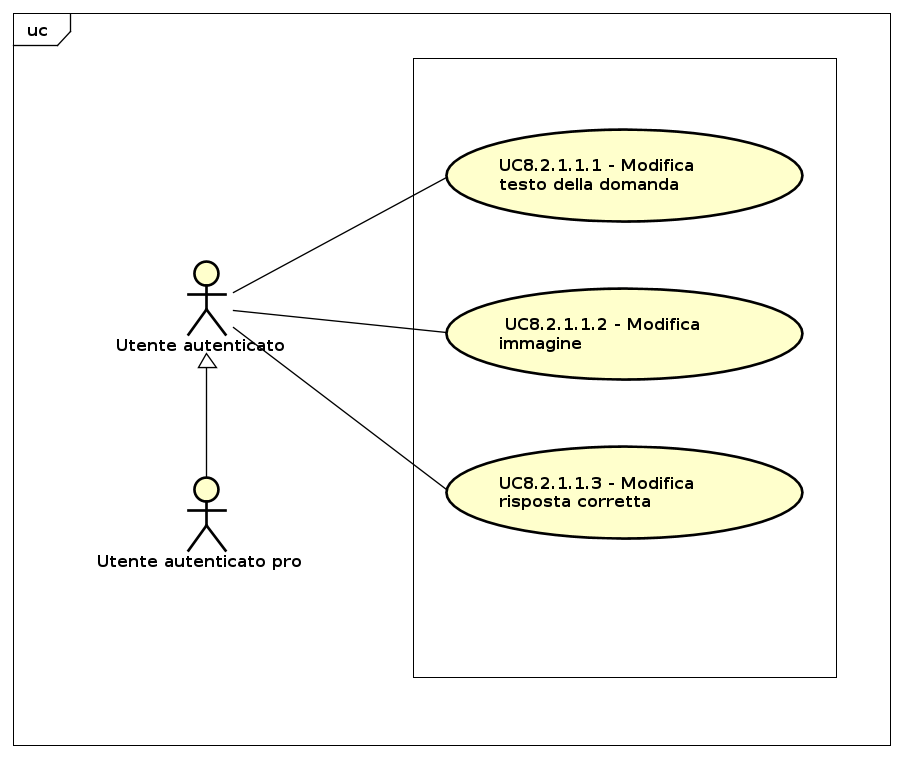
\includegraphics[scale=0.45,keepaspectratio]{UML/UC8_2_1_1.png}
		\caption{UC8.2.1.1: Modifica domanda vero/falso}
	\end{figure}
	\FloatBarrier
	\begin{itemize}
		\item
			\textbf{Attori}: utente autenticato, utente autenticato pro;
		\item		
			\textbf{Descrizione}: lo scopo di questa funzionalità è offrire agli attori la possibilità di modificare domande vero/falso;
		\item
			\textbf{Precondizione}: gli attori hanno selezionato la seguente funzionalità; 
		\item
			\textbf{Postcondizione}: gli attori hanno modificato una domanda vero/falso;
		\item
			\textbf{Scenario principale}:
	       		\begin{enumerate}
	       			\item
	       			Gli attori possono modificare il testo della domanda (UC8.2.1.1.1)
	       			\item
	       			Gli attori possono modificare l'immagine relativa al testo della domanda (UC8.2.1.1.2)
					\item
					Gli attori possono modificare la risposta corretta (UC8.2.1.1.3).
	 			\end{enumerate}
	\end{itemize}
	
\subsubsection{Caso d'uso UC8.2.1.1.1: Modifica testo della domanda}
	\begin{itemize}
		\item
			\textbf{Attori}: utente autenticato, utente autenticato pro;
		\item		
			\textbf{Descrizione}: lo scopo di questa funzionalità è offrire agli attori la possibilità di modificare il testo della domanda;
		\item
			\textbf{Precondizione}: gli attori hanno selezionato la funzionalità di modifica di una domanda vero/falso; 
		\item
			\textbf{Postcondizione}: gli attori hanno modificato il testo della domanda;
		\item
			\textbf{Scenario principale}: gli attori modificano il testo della domanda. 		
	\end{itemize}
	
\subsubsection{Caso d'uso UC8.2.1.1.2: Modifica immagine}
	\begin{itemize}
		\item
			\textbf{Attori}: utente autenticato, utente autenticato pro;
		\item		
			\textbf{Descrizione}: lo scopo di questa funzionalità è offrire agli attori la possibilità di modificare l'immagine relativa al testo della domanda;
		\item
			\textbf{Precondizione}: gli attori hanno selezionato la funzionalità di modifica di una domanda vero/falso; 
		\item
			\textbf{Postcondizione}: gli attori hanno modificato l'immagine;
		\item
			\textbf{Scenario principale}: gli attori modificano l'immagine. 	
	\end{itemize}
	
\subsubsection{Caso d'uso UC8.2.1.1.3: Modifica risposta corretta}
	\begin{itemize}
		\item
			\textbf{Attori}: utente autenticato, utente autenticato pro;
		\item		
			\textbf{Descrizione}: lo scopo di questa funzionalità è offrire agli attori la possibilità di modificare la selezione della risposta corretta;
		\item
			\textbf{Precondizione}: gli attori hanno selezionato la funzionalità di modifica di una domanda vero/falso; 
		\item
			\textbf{Postcondizione}: gli attori hanno modificato la selezione della risposta corretta;
		\item
			\textbf{Scenario principale}: gli attori modificano la selezione della risposta corretta. 
	 			
	\end{itemize}
	